\chapter{MIMO for Wireless MAN}
\author{Xiaopeng Fan, Steven Y. Lai, Yuan Zheng, and Jiannong Cao\\
Hong Kong Polytechnic University}

With the development of the last mile access in wireless networks,
Multiple-Input Multiple-Output (MIMO) has become one of the most
important technologies in Wireless Metropolitan Networks (WMANs),
which is based on WiMAX (Worldwide Interoperability for Microwave
Access) technology.  In this chapter, we discuss the relationship
between MIMO and Wireless MAN from three aspects, including the
capacity of MIMO, Space-time signal processing and the diversity
technique. For the first problem, we focus on the capacity of MIMO
systems in WiMAX, including a single user model and a multi-user
model. As for the space-time coding, we review most of codes in this
kind and then introduce the Alamouti code applied in WiMAX for IEEE
802.16-2004. We also described various diversity schemes for
enhancing the performance of wireless channels. Among them, Space
diversity is an effective scheme for combating multipath fading in
WiMAX. Finally, we conclude our chapter with a brief summary.

\section{Introduction}
As the possible next development in wireless IP offering a possible
solution to the last mile access problem, Wireless Metropolitan Area
Networks (WMANs) based on the 802.16 standards-based technology
\cite{6} have recently captured lots of interest from vendors and
ISPs. With a theoretical speed of up to 75 Mbps and a range of
several miles, 802.16 broadband is expected to be an alternative to
cable modem and DSL in the near future. Promoters of 802.16 have
elected to form an organization called the WiMAX (Worldwide
Interoperability for Microwave Access) Forum \cite{7} to test and
certify products for interoperability and standards compliance.

WiMAX specifies a technology devoted to making broadband wireless
commercially available to the mass market. WiMAX is an IEEE 802.16
standards-based technology, which supports point to multi-point
(PMP) broadband wireless access. The IEEE 802.16 specification
includes IEEE 802.16-2004 \cite{31} and 802.16e amendment \cite{6}
as the physical (PHY) layer specifications. The IEEE 802.16-2004
standard is primarily intended for stationary transmission while
IEEE 802.16e amendment is primarily intended for both stationary and
mobile deployments. Based on the IEEE 802.16-2004 Air Interface
Standard, fixed WiMAX has proven to be a cost-effective fixed
wireless alternative to cable and DSL services. Furthermore, the
IEEE ratified the 802.16e amendment \cite{6} to the 802.16 standard
in December 2005 to add the features and attributes to the standard
necessary for supporting mobility. The WiMAX Forum is now defining
system performance and certification profiles based on the IEEE
802.16e Mobile Amendment.

WiMAX is a wireless metropolitan area network technology that will
connect IEEE 802.11 (Wi-Fi) hotspots to the Internet and provide a
wireless extension to cable and DSL for last mile broadband access,
so it faces a lot of challenges in terms of coverage, data rate, and
mobility. For coverage, WiMAX is designed to provide up to 50 km of
linear service area and allow users connectivity without a direct
line of sight to a base station. For data rate, WiMAX should provide
enough bandwidth to simultaneously support more than 60 businesses
with T1-type connectivity and well over a thousand homes at the
1Mbit/s DSL-level connectivity. For mobility, WiMAX needs to support
a system of combined fixed and mobile broadband wireless access,
with subscriber stations moving at vehicular speeds and support. To
meet these new requirements, WiMAX adopts Multiple-Input
Multiple-Output (MIMO) and other new technologies. In this chapter,
we will focus on MIMO and its related technologies, including
Orthogonal Frequency Division Multiplexing (OFDM), Space-time
Coding, and diversity.

MIMO systems are a natural extension of developments in antenna
array communication \cite{1} \cite{2}. Sometimes referred to as
"volume-to-volume" wireless links, MIMO systems are important
because they have the potential to play a significant role in
resolving traffic capacity bottlenecks in future wireless networks.
Communication theory suggests that they can provide a potentially
very high capacity that, in many cases, would grow approximately
linearly with the number of antennas. Recently, MIMO systems have
attracted more and more attention because of their implementation in
wireless communication systems, especially in wireless MANs, and
because of the proposal of a number of different MIMO system
structures by industrial organizations in the Third Generation
Partnership Project (3GPP) standardizations.

MIMO systems can be simply defined as systems that contain multiple
transmitter antennas and multiple receiver antennas. As an example,
we might consider an arbitrary wireless communication system in
which the links on both the transmitting and receiving ends are
equipped with multiple antenna elements. The idea behind MIMO is
that the signals on the transmit (TX) antennas at one end and the
receive (RX) antennas at the other end are "combined" in such a way
as to improve the quality (Bit Error Rate) or the data rate
(bits/sec) of the communication for each MIMO user. This has
significant advantages in terms of both the network's quality of
service and the operator's revenues.

When we analyze the capacity of MIMO, it is important to note that
OFDM is particularly well suited to MIMO technology. OFDM is a
multiplexing technique that subdivides bandwidth into multiple
frequency sub-carriers \cite{8}. In an OFDM system, the input data
stream is divided into several parallel sub-streams of reduced data
rate (thus increased symbol duration) and each sub-stream is
modulated and transmitted on a separate orthogonal sub-carrier.
Because the narrowband subcarriers in the OFDM signal experience
flat fading, MIMO reception does not require complex channel
equalization schemes. So when we discuss the capacity of the
multi-user MIMO-OFDM system in Section 2 , the basic ideas of OFDM
will be introduced.

Space-time signal processing \cite{29} is one of the core ideas in
MIMO. This involves complementing the use of time, the natural
dimension of digital communication data, with the use of the spatial
dimension inherent in the use of multiple spatially distributed
antennas. Space-Time Codes (STCs) \cite{5} is used for coding
signals in both the temporal and spatial domains. MIMO systems can
also be viewed as an extension of the so-called smart antennas, a
popular technology using antenna arrays for improving wireless
transmission dating back several decades.

Multi-path fading is a significant problem in MIMO communications
\cite{10}. In a fading channel, signal strength will decrease
significantly, leading to a failure to receive signals. One way to
combat fading is to make use of diversity \cite{11}, which can take
full advantage of the redundancy of the signals over time,
frequency, or space on the transmitting and receiving terminals. In
general, the effectiveness of any diversity technique is guaranteed
by the fact that the receiver can provide independent samples of the
basic signal that was transmitted. Based on this, we can assume that
two or more relevant parts of a signal will not fade significantly
at the same time. To achieve great improvements in the quality of
signals, diversity techniques need to optimally fuse the received
diversified samples. Thus, depending on the signal domain which was
the source of the redundancy, diversity techniques are classified as
either time, frequency, or space diversity.

This chapter is organized as follows. In Section 2, we analyze the
capacity of MIMO systems to understand how much MIMO improves the
capacity when used in WiMAX. We begin this work with a single user
MIMO system model and highlight the capacity analysis under two
different physical specifications in WiMAX. In Section 3, we discuss
various kinds of space-time block codes (STBCs) used in MIMO and how
they are applied in WiMAX. In Section 4, we discuss the diversity
technique to know how much MIMO improves the reliability in WiMAX.
In the last section, we conclude our chapter with a brief summary.

\section{Multiple-Input Multiple-Output Wireless Communication}

In this section, we begin with a single user MIMO system model.
Based on the model, we generalize the discussion on capacity to
cases that encompass transmitters having some prior knowledge of a
channel \cite{9}. Then we consider a single MIMO user communicating
over a fading channel with additive white Gaussian noise (AWGN).
Finally we discuss the capacity of MIMO systems in WiMAX, including
a multi-user model.

\subsection{MIMO System Model}

A single user MIMO system consists of $n_{T}$ transmitter antennas
(Tx) and $n_{R}$ receiver antennas (Rx). During each Symbol Time
Slot (STS), the transmitted signals are presented as an
$n_{T}\times1$ column vector $x$, whose entry $x_{i}$,
$i=1,...,n_{T}$, is the transmitted signal at the $i^{th}$ Tx
antenna during the considered STS. Figure \ref{fig:Fig1} is a
diagram of a wireless transmission system. The transmitter and
receiver are equipped with multiple antenna elements. Coding,
modulation, and mapping of the signals onto the antennas may be
realized jointly or separately.

We consider here an additive Gaussian MIMO channel for which the
optimal distribution of the transmitted signals in $x$ is also
Gaussian, i.e., the transmitted signals $x_{i}$, for
$i=1,...,n_{T}$, are zero-mean, identically independently
distributed (i.i.d.) complex random variables. The covariance matrix
of $x$ is $R_{xx}=E\{xx^{H}\}$, where $E\{.\}$ denotes the
expectation, and $(.)^{H}$ denotes the Hermitian transposition
operation, i.e. the transpose-conjugate operation. The total power
of transmitted signals (during each STS) is constrained to $P$,
regardless of the number of transmitter antennas $n_{T}$. This
implies that $P=tr(R_{xx})$ where $tr(.)$ denotes the trace
operation on the argument matrix.

In all following sections, we assume that channel coefficients (or
transmission coefficients) are perfectly known at the receiver, but
may or may not be known at the transmitter.

When channel coefficients are unknown at the transmitter (but known
at the receiver), we assume that the transmitted power at each Tx
antenna is the same and equal to $P_{tj}=\frac{P}{n_{T}}$, for
$j=1,...,n_{T}$. When the channel coefficients are known at the
transmitter, the transmitted power is unequally assigned to the Tx
antennas following the water-filling rule \cite{13}. The scenario
where channel coefficients are unknown at both transmitter and
receiver is mentioned in \cite{12}. Most of the results in this
section can be found in \cite{30}.

The channel is represented by an $n_{R}\times n_{T}$ complex matrix
$H$, whose elements $h_{ij}$ are the channel coefficients between
the $j^{th}$ Tx antenna ($j=1,...,n_{T}$) and the $i^{th}$ Rx
antenna $i=1,...,n_{R}$. Channel coefficients $h_{ij}$ are assumed
to be zero-mean, i.i.d. complex Gaussian random variables with a
distribution $CN(0,1)$. Noise at the receiver is represented by an
$n_{R} \times 1$ column vector $n$ whose elements are zero-mean,
i.i.d. complex Gaussian random variables with identical variances
$\sigma^{2}$.

Let $r$ denote the column vector of signals received at $R_{x}$
antennas during each STS, the transmission model is represented as
follows.
\[ r = Hx + n \]

If we assume that the average total power $P_{r}$ received by each
Rx antenna (regardless of noise) is equal to the average total
transmitted power $P$ from $n_{T}$ Tx antennas, the Signal-to-Noise
(SNR) at each Rx antenna is given by the following equation
\[\rho=\frac{P_{r}}{\sigma^{2}}=\frac{P}{\sigma^{2}}\]

To guarantee the assumption that , for a channel with fixed channel
coefficients and the equal transmitted power per Tx antenna
$P/n_{T}$ (i.e., channel coefficients are known at the receiver, but
unknown at the transmitter), we have the following constraint:
\begin{equation}
 \sum_{j=1}^{n_{T}}|h_{ij}|^{2}=n_{T}
\end{equation}
for $i=1,...,n_{R}$. For a channel with random channel coefficients
and equal transmitted power per Tx antenna, Formula (2.1) is
calculated with the expected value.

The system capacity $C(bits/s)$ is defined as the maximum possible
transmission rate such that the error probability is arbitrarily
small. In this chapter, we also consider the normalized capacity
$C/W(bits/s/Hz)$, which is the system capacity $C$ normalized to the
channel bandwidth $W$.

\subsection{Capacity of MIMO}
In this section, we consider the Additive Gaussian Noise Channels
with fixed channel coefficients. We derive the most general formula
to calculate the channel capacity for both cases where channel
coefficients are known as well as unknown at the transmitters.

The general formula for calculating the channel capacity in the case
where channel coefficients are either known or unknown at the
transmitter is give by the Shannon capacity:
\begin{equation}
 C=W\sum_{i=1}^{r}log_{2}(1+\frac{P_{ri}}{\sigma^{2}})
\end{equation}
where $W$ is the bandwidth of each sub-channel, $r$ is the rank of
the channel coefficient matrix $H$($r$ is equal to the number of
non-zero eigenvalues of $H^{H}H$), $P_{ri}$ is the received power at
each Rx antenna from the $i^{th}$ sub-channel, for $i=1,...,r$,
during the symbol time slot under consideration . The rank $r$ is
less than or equal to $m=min(n_{T},n_{R})$.

Then, we calculate the channel capacity where there are unknown
channel coefficients at the transmitter. Let $Q$  be the Wishart
matrix defined as
\[f(n) = \left\{
\begin{array}{l l}
  HH^{H}& \quad \mbox{if $n_{R}<n_{T}$}\\
  H^{H}H & \quad \mbox{if $n_{R}\geq n_{T}$}\\ \end{array} \right. \]
From Eq. (2.2), it has been proved in \cite{13} that the channel
capacity for such a scenario is
\begin{equation}
C=Wlog_{2}[det(I_{r}+\frac{\rho}{n_{T}}Q)]
\end{equation}
where $det(.)$ denotes the determinant of the argument matrix.

The channel capacity can be increased if channel coefficients are
known at the transmitter. In that case, the transmitted power is
assigned unequally to the Tx antennas, according to the
"water-filling" rule, i.e., a larger power is assigned to a better
sub-channel and visa versa (see Appendix 1.1 in \cite{13}). The
power assigned to the $i^{th}$ sub-channel is
\[P_{ti}=(\mu-\frac{\sigma^{2}}{\lambda_{i}})^{+} \quad i=1,...,r\]
where $(a)^{+}=\max(a,0)$, $\lambda_{i}$ is the non-zero eigenvalues
of the matrix $H^{H}H$(also $HH^{H}$) and $\mu$ is determined to
satisfy the power constraint
\begin{equation}
\sum_{i=1}^{r}P_{ti}=P
\end{equation}
For the $i^{th}$ sub-channel, the received power $P_{ri}$ at the
receiver antenna is calculated as (see Eq. (1.20) in \cite{13}):
\[P_{ri}=\lambda_{i}P_{ti}=(\lambda_{i}\mu-\sigma^{2})^{+}\]
Then, the channel capacity is given below:
\begin{equation}
C=W\sum_{i=1}^{r}log_{2}[1+\frac{(\lambda_{i}\mu-\sigma^{2})^{+}}{\sigma^{2}}]
\end{equation}

\subsection{Capacity of MIMO in WiMAX}

As mentioned before, WiMAX technology is based on the IEEE 802.16
specification, which includes IEEE 802.16-2004 \cite{31} and 802.16e
amendment as the Physical (PHY) layer specifications. The IEEE
802.16-2004 standard is primarily intended for stationary
transmission while 802.16e amendment is primarily intended for both
stationary and mobile deployments. In this section, we will examine
the PHY layer in WiMAX in detail. We discuss two different physical
layer specifications in \cite{6}.

The 10-66 GHz bands provide a physical environment where, due to the
short wavelength, line-of-sight (LOS) is required and multipath is
negligible. In the 10-66 GHz band, channel bandwidths of 25 MHz or
28 MHz are typical. With raw data rates in excess of 120 Mb/s, this
environment is well suited for PMP (Point to Multipoint) access
serving applications from small office/home (SOHO) through medium to
large office applications.

In the design of the physical layer for 10-66 GHz, line-of-sight
propagation was deemed a practical necessity. With this condition
assumed, single-carrier modulation was easily selected; the air
interface is designated as "WirelessMAN-SC." However, many
fundamental design challenges remained. Because of the
point-to-multipoint architecture, the BS basically transmits a TDM
signal, with individual subscriber stations allocated time slots
serially. Access in the uplink direction is by Time-Division
Multiple Access (TDMA). Following extensive discussions regarding
duplexing, a burst design was selected that allows simultaneously
both time-division duplexing (TDD), in which the uplink and downlink
share a channel but do not transmit simultaneously, and
frequency-division duplexing (FDD), in which the uplink and downlink
operate on separate channels, sometimes simultaneously. This burst
design allows both TDD and FDD to be handled in a similar fashion.
Support for half-duplex FDD subscriber stations, which may be less
expensive since they do not simultaneously transmit and receive, was
added at the expense of some slight complexity. Both TDD and FDD
alternatives support adaptive burst profiles in which modulation and
coding options may be dynamically assigned on a burst-by-burst
basis.

In the above scenario, the channel model can be modeled as the flat
Rayleigh Fading channel. We assume that channel coefficients are
zero-mean, i.i.d. complex Gaussian random variable with variance of
1/2 per dimension (real and imaginary).  Hence, each channel
coefficient has a Rayleigh distributed magnitude, uniformly
distributed phase and the expected value of the squared magnitude
equal to one, i.e., $E\{|h_{i,j}^{2}|=1\}$. In all following
sections, channel coefficients are assumed to be known at the
receiver, but unknown at the transmitter. Thus, the transmitted
power per Tx antenna is assumed to be identical and equal to
$P_{tj}=\frac{P}{n_{T}}$, for $j=1,...,n_{T}$.

If the channel coefficient matrix $H$ is random and its entries
change randomly during every symbol time slot (STS), then the
channel is referred to as the fast flat Rayleigh fading channel. The
capacity of MIMO systems in fast and block Rayleigh fading channels
is calculated as follows (see Eq. (1.56) in \cite{13} or Theorem 1
in [19 Telatar, 1999])
\begin{equation}
C=E\{W\log_{2}[det(I_{r}+\frac{P}{n_{T}\sigma^{2}})Q]\}
\end{equation}
where $r$ is the rank of matrix $H$ and the matrix $Q$ is the
Wishart matrix defined above.

If $H$ is random and its entries change randomly after each block
containing a fixed number of STSs, then the channel is referred to
as the block flat Rayleigh fading channel. If $H$ is random but is
selected at the beginning of transmission and its entries keep
constant during the whole transmission, the channel is referred to
as the slow flat Rayleigh fading channel. These results were
originally derived by Foschini and Gans \cite{9}. Considering a MIMO
system where the channel coefficient matrix $H$ is chosen randomly
at the start of transmission and says constant during the whole
transmission. The entries of $H$ follow the Rayleigh distribution.
Examples of this scenario include Wireless Local Area Networks
(LANs) with high data rates and low fade and 802.16 for fix
broadband access systems in Wireless Metropolitan Areas Networks
(WMANs).

Now, we consider the transmit and receive diversity. We first assume
that $n=n_{T}=n_{R}$ and $n$ is large. As shown by Eq. (20) in
\cite{9} or by Eq. (1.82) in \cite{13}, the lower bound on the
capacity is given by
\begin{equation}
\frac{C}{W_{n}}>(1+\frac{\sigma^{2}}{P})\log_{2}(1+\frac{P}{\sigma^{2}})-\log_{2}e+\varepsilon_{n}
\end{equation}
Where $\varepsilon_{n}$ is a Gaussian random variable with the mean
and variance as given below:
\[E\{\varepsilon_{n}\}=\frac{1}{n}\log_{2}(1+\frac{P}{\sigma_{2}})^{-1/2}\]
\[Var\{\varepsilon_{n}\}=(\frac{1}{n\ln2})^{2}[ln(1+\frac{P}{\sigma^{2}})-\frac{\frac{P}{\sigma^{2}}}{1+\frac{P}{\sigma^{2}}}] \]

The other bands, frequencies below 11 GHz, provide a physical
environment where, due to the longer wavelength, LOS is not
necessary and multipath may be significant. The ability to support
near-LOS and non-LOS (NLOS) scenarios requires additional PHY
functionality, such as the support of advance power management
techniques, interference mitigation/coexistence, and multiple
antennas.

The original WiMAX standard (IEEE 802.16) specified WiMAX in the 10
to 66 GHz range. 802.16a, updated in 2004 to 802.16-2004 (also known
as 802.16d), added support for the 2 to 11 GHz range. 802.16d was
updated to 802.16e in 2005. Revision 802.16e uses scalable OFDM as
opposed to the non-scalable version used in revision 802.16d. This
brings potential benefits in terms of coverage, self installation,
power consumption, frequency re-use and bandwidth efficiency.
Revision 802.16e also adds a capability for full mobility support.
Design of the 2-11 GHz physical layer is driven by the need for
non-line-of-sight (NLOS) operation. Because residential applications
are expected, rooftops may be too low for a clear sight line to a BS
antenna, possibly due to obstruction by trees. Therefore,
significant multipath propagation must be expected.

IEEE 802.16-2005 (formerly named, but still best known as, 802.16e
or Mobile WiMAX) provides an improvement on the modulation schemes
stipulated in the original (fixed) WiMAX standard. It allows for
fixed wireless and mobile NLOS applications primarily by enhancing
the Orthogonal Frequency Division Multiple Access (OFDMA).
Furthermore, outdoor-mounted antennas are expensive due to both
hardware and installation costs. The three 2-11 GHz air interface
specifications \cite{15} are:
\begin{itemize}
\item
WirelessMAN-SCa: It uses a single-carrier modulation format.
\item
WirelessMAN-OFDM: It uses orthogonal frequency-division multiplexing
with a 256-point transform. Access is by TDMA. This air interface is
mandatory for license exempt bands.
\item
WirelessMAN-OFDMA: It uses orthogonal frequency-division multiple
access with a 2048-point transform. In this system, multiple access
is provided by addressing a subset of the multiple carriers to
individual receivers.
\end{itemize}

OFDM has become a popular technique for transmission of signals over
wireless channels. It converts a frequency-selective channel into a
parallel collection of frequency flat subchannels, which makes the
receiver simpler. The time domain waveforms of the subcarriers are
orthogonal, yet the signal spectra corresponding to different
subcarriers overlap in frequency. Hence, the available bandwidth is
used very efficiently. Using adaptive bit loading techniques based
on the estimated dynamic properties of the channel, the OFDM
transmitter can adapt its signaling to match channel conditions, and
approach the ideal water pouring capacity of a frequency-selective
channel. The increased symbol duration improves the robustness of
OFDM to delay spread. Furthermore, the introduction of the cyclic
prefix (CP) can completely eliminate Inter-Symbol Interference (ISI)
as long as the CP duration is longer than the channel delay spread.
The CP is typically a repetition of the last samples of data portion
of the block that is appended to the beginning of the data payload.

MIMO is known to boost capacity. For high-data-rate transmission,
the multipath characteristic of the environment causes the MIMO
channel to be frequency-selective.  OFDM can transform such a
frequency-selective MIMO channel into a set of parallel
frequency-flat MIMO channels, and therefore decrease receiver
complexity. The combination of the two powerful techniques, MIMO and
OFDM, is very attractive and has become one of the most promising
broadband wireless access schemes. In the following, we will
consider the capacity of MIMO-OFDM.

In the scheme proposed in \cite{14}, at transmitter, the bit streams
for each of $n_{T}$ antennas are coded separately and then mapped to
their corresponding symbols. These symbols are then grouped into
$N_{F}$ symbols with a serial to parallel (S/P) converter and spread
with a $N_{C}$ size Walsh spreading codes, where $N_{F}>N_{C}$.
Next, $N_{F}$ point IFFT is performed and time domain symbols are
parallel to serial (P/S) converted and transmitted. At receiver,
$n_{R}$ antennas receive signals from user $k$ and pass them through
a complex channel matrix whose characteristic is described by the
independent identically distributed (i.i.d.) complex Gaussian random
matrix $H_{k}$. In all the following cases, we assume that the
realization of $H_{k}$ is known to the receiver perfectly but
unknown to the transmitter. $L$ is defined as the maximum number of
interfered symbols corresponding with maximum delay spread. Thus,
the channel matrix of user $k$, $\tilde{H}_{k}$, is written as
\[ \tilde{H}_{k}= \left[ \begin{array}{cccc}
H_{k}^{1} & 0 & \cdots & 0 \\
\vdots & H_{k}^{1} & \cdots & 0 \\
H_{k}^{L} & \vdots & \ddots & 0 \\
0 & H_{k}^{L} & \ddots & H_{k}^{1} \\
0 & 0 & \ddots & \vdots \\
0 & 0 & \cdots & H_{k}^{L} \end{array} \right].\]

For a single user channel in MIMO-OFDM, we can calculate the
capacity of the considered system as
\begin{equation}
C=E[\log_{2}det(I_{m}+\frac{\rho}{n_{T}}\tilde{H}_{k}^{''}\tilde{H}_{k}^{''+})]
\end{equation}
where $E[]$denotes expectation, $m$ is $\min(n_{R},n_{T})$ and
$\rho$ is an average signal to noise ratio (SNR) at each receive
antenna. $H^{T}$ denotes transpose of matrix $H$, $H^{+}$ denotes
conjugate and transpose of matrix $H$.

For a multi-user channel in MIMO-OFDM, we can calculate the capacity
considered system as
\begin{equation}
C=\bigcup\{(R_{1},...,R_{K}):\sum_{i\in S}{R_{i}}\leq
E[\log_{2}det(I_{m}+\sum_{i\in
S}\frac{\rho}{n_{T}}\tilde{H}_{i}^{''}\tilde{H}^{''+})]\}
\end{equation}
where $K$ is the number of users, $\forall S\subseteq\{1,2,...,K\}$
. We assume that the receiver knows the realization of every user
matrix channel. Also we assume that all the transmitting devices
generate equal power and use the same number of antennas.

\section{Space-Time Block Codes}
A space-time block code (STBC) is a channel coding method used in
multiple-antenna wireless communications. The objective of STBC is
to improve the reliability of high data rate transmission in
wireless communication systems by transmitting multiple, redundant
copies of a data stream in the hope that some of them may arrive at
the receiver in a better state than others.

Most of the earlier works on wireless communications had focused on
having an antenna array at only one end of the wireless link -
usually at the receiver. Then, some works extended the scope of
wireless communication possibilities by showing that substantial
capacity gains are enabled when antenna arrays are used at both ends
of a link. Examples are D-BLAST \cite{15} and V-BLAST \cite{16}.
Later, space-time code \cite{5} (STC) was proposed as an alternative
approach which relies on having multiple transmit antennas and only
optionally multiple receive antennas. It has been shown that STC
achieves significant error rate improvements over single-antenna
systems. Its original scheme was based on trellis codes. However,
the cost for this scheme is additional processing, which increases
exponentially as a function of bandwidth efficiency (bits/s/Hz) and
the required diversity order. A simpler approach called block codes
was proposed by Siavash Alamouti \cite{11}, and later extended to
develop space-time block-codes (STBCs) \cite{17}.

An STBC is usually represented by a matrix. Each row represents a
time slot and each column represents one antenna's transmissions
over time.

%Problem with arrow above the matrix
%\[
%\stackrel{transmit\;antennas} { \stackrel{\rightarrow} {time-slots
%\left\downarrow \left[
%\begin{array}{cccc}
%s_{11} & s_{12} & \cdots & s_{1nT}\\
%s_{21} & s_{22} & \cdots & s_{2nT}\\
%\vdots & \vdots & \ddots & \vdots \\
%s_{r1} & s_{r2} & \cdots & s_{rnT}\\
%\end{array}
%\right]\right. }}
%\]
\[
time\;slots \stackrel{transmit\;antennas} { \overrightarrow{
\left\downarrow \left[
 \begin{array}{cccc}
 s_{11} & s_{12} & \cdots & s_{1nT}\\
 s_{21} & s_{22} & \cdots & s_{2nT}\\
 \vdots & \vdots & \ddots & \vdots \\
 s_{r1} & s_{r2} & \cdots & s_{rnT}\\
 \end{array} \right]
\right. } }
\]
Here, $s_{ij}$ is the modulated symbol to be transmitted in time
slot $i$ from antenna $j$. There are $T$ time slots and $nT$
transmit antennas as well as $nR$ receive antennas.

The code rate of an STBC measures how many symbols per time slot it
transmits on average over the course of one block \cite{17}. If a
block encodes $k$ symbols, the code-rate is
\[r=\frac{k}{T}\]
\begin{itemize}
\item Alamouti's Code: Alamouti invented the simplest of all the STBCs \cite{11}. It was designed for a two transmit antenna system and has the coding matrix:
\[C_2=
\left[\begin{array}{cc}
s_1 & s_2\\
-s_2^* & -s_1^*
\end{array} \right]\]
where $*$ denotes complex conjugate.

It is readily apparent that this is a full-rate code. It takes two
time-slots to transmit two symbols and the bit-error rate (BER) of
this STBC is equivalent to $2nR$-branch maximal ratio combining
(MRC). This is a result of the perfect orthogonality between the
symbols after the receive processing - there are two copies of each
symbol transmitted and $nR$ copies received.

\item Higher order STBCs: Tarokh et al. discovered a set of higher order STBCs \cite{17, 18}. They also proved that no code for more than two transmit antennas could achieve full-rate. Their codes have since been improved upon (both by the original authors and by many others). Nevertheless, they serve as clear examples of why the rate cannot reach one, and what other problems must be solved to produce 'good' STBCs. They also demonstrated the simple, linear decoding scheme that goes with their codes under the perfect channel state information assumption.

Two STBCs for 3 transmit antennas are:
\[
C_{3,1/2}= \left[\begin{array}{ccc}
s_1 & s_2 & s_3\\
-s_2 & s_1 & s_4\\
-s_3 & s_4 & s_1\\
-s_4 & -s_3 & s_2\\
s^*_1 & s^*_2 & s^*_3\\
-s^*_2 & s^*_1 & s^*_4\\
-s^*_3 & s^*_4 & s^*_1\\
-s^*_4 & -s^*_3 & s^*_2
\end{array} \right] \;and\; C_{3,3/4}=
\left[\begin{array}{ccc}
s_1 & s_2 & \frac{s_3}{\sqrt{2}}\\
-s^*_2 & s^*_1 & \frac{s_3}{\sqrt{2}}\\
\frac{s^*_3}{\sqrt{2}} & \frac{s^*_3}{\sqrt{2}} & \frac{(-s_1-s^*_1+s_2-s^*_2)}{2}\\
\frac{s^*_3}{\sqrt{2}} & -\frac{s^*_3}{\sqrt{2}} &
\frac{(s_2+s^*_2+s_1-s^*_1)}{2}
\end{array} \right]
\]
These codes achieve the rates of $1/2$ and $3/4$ respectively. The
two matrices give examples of why codes for more than two antennas
must sacrifice rate - it is the only way to achieve orthogonality.
One particular problem with   is that it has uneven power among the
symbols it transmits. This means that the signal does not have a
constant envelope and the power that each antenna must transmit has
to vary, both of which are undesirable. Modified versions of this
code that overcome this problem have since been designed.

Two STBCs for four transmit antennas are:
\[
C_{4,1/2}= \left[\begin{array}{cccc}
s_1 & s_2 & s_3 & s_4\\
-s_2 & s_1 & s_4 & s_3\\
-s_3 & s_4 & s_1 & -s_2\\
-s_4 & -s_3 & s_2 & s_1\\
s^*_1 & s^*_2 & s^*_3 & s^*_4\\
-s^*_2 & s^*_1 & s^*_4 & s^*_3\\
-s^*_3 & s^*_4 & s^*_1 & -s^*_2\\
-s^*_4 & -s^*_3 & s^*_2 & s^*_1
\end{array} \right] \;and\; C_{4,3/4}=\left[\begin{array}{cccc}
s_1 & s_2 & \frac{s_3}{\sqrt{2}} & \frac{s_3}{\sqrt{2}}\\
-s^*_2 & s^*_1 & \frac{s_3}{\sqrt{2}} & -\frac{s_3}{\sqrt{2}}\\
\frac{s^*_3}{\sqrt{2}} & \frac{s^*_3}{\sqrt{2}} & \frac{(-s_1-s^*_1+s_2-s^*_2)}{2} & \frac{(-s_2-s^*_2+s_1-s^*_1)}{2}\\
\frac{s^*_3}{\sqrt{2}} & -\frac{s^*_3}{\sqrt{2}} & \frac{(s_2+s^*_2+s_1-s^*_1)}{2} & \frac{(s_1+s^*_1+s_2-s^*_2)}{2}\\
\end{array} \right]
\]
These codes achieve the rates of $1/2$ and $3/4$ respectively, as
for their 3-antenna counterparts. $C_{4,3/4}$ exhibits the same
uneven power problems as $C_{3,3/4}$. An improved version of
$C_{4,3/4}$ is \cite{19}:
\[
C_{4,3/4}=\left[\begin{array}{cccc}
s_1 & s_2 & s_3 & 0\\
-s^*_2 & s^*_1 & 0 & s_3\\
-s^*_3 & 0 & s^*_1 & -s_2\\
0 & -s^*_3 & s^*_2 & s_1
\end{array} \right]
\]
which has equal power from all antennas in all time-slots.
\end{itemize}
\subsection{Orthogonal Space-Time Block Codes}
STBCs, as originally introduced are orthogonal , meaning that the
STBC is designed in such a way that the vectors representing any
pair of columns taken from the coding matrix are orthogonal. The
result of this is simple, linear, optimal decoding at the receiver.
Its most serious disadvantage is that all but one of the codes that
satisfy this criterion must sacrifice some proportion of their data
rate.

There are also 'quasi-orthogonal STBCs' that allow some inter-symbol
interference but can achieve a higher data rate, and even a better
error-rate performance, in harsh conditions. Quasi-orthogonal STBCs
exhibit partial orthogonality and provide only part of the diversity
gain. An example given by Hamid Jafarkhani in \cite{20} is:
\[
C_{4,1}=\left[\begin{array}{cccc}
s_1 & s_2 & s_3 & s_4\\
-s^*_2 & s^*_1 & -s^*_4 & s^*_3\\
-s^*_3 & -s^*_4 & s^*_1 & s^*_2\\
s_4 & -s_3 & -s_2 & s_1
\end{array} \right]
\]
The orthogonality criterion only holds for columns (1 and 2), (1 and
3), (2 and 4) and (3 and 4). Crucially, however, the code is
full-rate and still only requires linear processing at the receiver,
although decoding is slightly more complex than for orthogonal
STBCs. Results show that this Q-STBC outperforms (in a bit-error
rate sense) the fully-orthogonal 4-antenna STBC over a good range of
signal-to-noise ratios (SNRs). At high SNRs, though (above about
22dB in this particular case), the increased diversity offered by
orthogonal STBCs yields a better BER. Beyond this point, the
relative merits of the schemes have to be considered in terms of
useful data throughput. More Q-STBCs have also been developed
considerably from the basic example shown above.
\subsection{Space-Time Block Codes for WiMAX}
In IEEE 802.16-2004 OFDM-256, the Alamouti code is applied to a
specific subcarrier index $k$. For instance, suppose that in the
uncoded system $S_1[k]$ and $S_2[k]$ are sent in the first and
second OFDM symbol transmissions.  The Alamouti encoded symbols send
$S_1[k]$ and $S_2[k]$ off the first and second antennas in the first
transmission and $-S_2^*[k]$ and $S_1^*[k]$ off the first and second
antennas in the next transmission.

There are a number of features of IEEE 802.16-2004 OFDM-256 Alamouti
transmission that are of interest.  The first is that the preamble
for Alamouti transmission is transmitted from both antennas with the
even subcarriers used for antenna 1 and the odd subcarriers used for
subcarrier 2. This means that each set of data needs to be
appropriately smoothed, which is done in these simulations. The
second feature is that the pilots have certain degenerate
situations: for the first Alamouti transmitted symbol, the pilots
destructively add and for the second Alamouti transmitted symbol,
the pilots constructively add. Hence, the pilots are not always
useful. The pilot symbols must be processed properly.

Figure \ref{fig:Fig2} shows the detailed flow of an Alamouti
implementation \cite{21}. This implementation has two parts. The
first calculates the parameters that are necessary for data
demodulation such as channel estimates. The second part is the
actual data demodulation and tracking. It has been shown that under
various conditions, the error rates can be greatly reduced when the
Alamouti Code is used.


\section{Transmission Diversity Techniques}
A key feature of MIMO systems is their ability to turn multipath
propagation, traditionally a pitfall of wireless transmission, into
a user benefit \cite{3}. MIMO effectively multiplies transfer rates
by taking advantage of random fading and, when available, multipath
delay spread. This prospect of an improvement in wireless
communication performance of many orders of magnitude at no extra
spectrum cost (adding only hardware and complexity) largely accounts
for the success of MIMO as a new technology. It  and has prompted
progress in areas as diverse as channel modeling, information theory
and coding, signal processing, antenna design, and fixed and mobile
multiantenna-aware cellular design.

\subsection{Time Diversity}
Time diversity is a diversity technique where identical signals are
transmitted during different time slots. Because the channel must
provide sufficient variations in time, the time slots can be
uncorrelated, i.e. the temporal separation between those slots is
greater than the coherence time of the wireless channel \cite{22}.
Thus, the interleaving symbol duration is independent of the
previous symbol and then, the completely new replica of the original
signal can be obtained.

However, this technique will incur considerable redundancy in the
time domain, which will cause a negative consequence of a loss in
bandwidth efficiency. The loss in bandwidth is due to the guarantee
of time duration being larger than coherence time between the time
slots. In practice, interleavers and error control coding, such as
Forward Error Correction (FEC) codes, are applied to provide time
diversity for the receiver. In addition, RAKE receiver in CDMA (Code
Division Multiple Access) system is also an example of the modern
implementation of time diversity is the RAKE receiver in CDMA (Code
Division Multiple Access) systems \cite{10}.

\subsection{Frequency Diversity}
The frequency diversity technique uses several carriers with
different frequencies to transmit the same signals. The frequency
separation between these carrier frequencies is an order of several
times of the coherence bandwidth of the channel to achieve
uncorrelated carriers, which do not experience the same fades. As in
time diversity, in frequency diversity, the redundancy in the
frequency domain will lead to a loss in spectral efficiency. The
loss in spectral efficiency is aiming to guarantee the enough
spectral bands existing among the carrier frequencies without
coherence \cite{23}. Additionally, the receivers need to employ
complicated receiving devices which can work with a number of
frequencies. In practice, frequency diversity is often used in
Line-Of-Sight (LOS) microwave channels. Some examples of systems
employing frequency diversity include spread spectrum systems, such
as Direct Sequence Spread Spectrum (DS-SS), Frequency Hop Spread
Spectrum (FH-SS) or Multi-Carrier Spread Spectrum (MC-SS) systems
\cite{10}.

\subsection{ Space Diversity}
Space diversity techniques, also named antenna diversity techniques,
use multiple transmitting and receiving antennas to transmit and/or
receive signals \cite{3}. These antennas are installed with at least
coherent distance among each other, where a coherent distance is a
half of wavelength of a signal. The requirement of spatial distance
allows every involved antenna to be regarded as an independent
sampling channel \cite{26}.

Different from time diversity and frequency diversity, the
redundancy incurred by spatial diversity is provided for the
receiver in the spatial domain. Therefore, these techniques will not
cause a loss in spectral or bandwidth efficiency. However, space
diversity needs a larger space to install multiple interference-free
antennas at the transmitters and receivers compared with the time
and frequency techniques.

In practical wireless communication systems, space diversity
techniques are often combined with other diversity techniques to
achieve multi-dimensional diversity. For instance, in MIMO systems
\cite{3}, a combination between multiple antennas at the base
station (space diversity) and time coding (time diversity) is
utilized to provide the 2-dimensional diversity for receivers
(mobile users) \cite{10}.

The spatial diversity techniques can be further classified according
to different criteria. Depending on how the redundant signals are
combined at the receivers, space diversity techniques are classified
into selection combining technique \cite{24}, maximum ratio
combining (MRC) technique \cite{11}, scanning combining technique
\cite{25}, equal-gain combining technique\cite{25}. Depending on
whether a technique is applied to the transmitter or to the
receiver, it can be classified as using either transmit diversity or
receive diversity \cite{29}. Depending on how the replicas of the
transmitted signals are combined at the receiver. In additional,
there are also three other techniques, including polarization
diversity \cite{27}, angle diversity \cite{28}. In following part of
this section, we will give a description of them in detail.

\subsubsection{Combination Techniques for Space Diversity}
In this part, we will introduce four important space diversity
combination techniques:  selection combining, switch combining,
equal-gain combining, and maximum ratio combining. All of them are
designed to achieve a high diversity gain, which means that the
combination replicas of signals can effectively improve the signal
transmission in channels. In order to achieve diversity gains, three
important conditions have to be satisfied, as listed below:
\begin{itemize}
\item
Redundancy: the identical signal should be transmitted at different
communication channels.
\item
Distinction: the signals transmitted in the different channels can
be distinct at a receiver without significant distortion.
\item
Independence: the channels carrying the identical signal should have
statistically different fading parameters.
\end{itemize}

Selection combining is the simplest spatial diversity combining
method. It requires only an SNR monitoring action and an antenna
switch at the receiver. In this technique, the receiver needs M
antennas and demodulators to provide M branches of signal samplings.
The receiver selects the incoming signal sampling with the highest
SNR to demodulate at every sampling instant. In practice, because
the instantaneous SNR is difficult to measure, as a substitution, it
measures the signals with the highest strength (including the
strength of both the signal and the noise).

Obviously, the SNR of the received signals is larger than the
average SNR of all signals provided by all pairs of antennas and
demodulators, since the signal with the highest SNR will be selected
in every sampling instant. However, this technique has not taken
full advantage of the total diversified signals simultaneously to
provide the best received signals. Thus, this technique is not the
optimal method for combining signals.

Maximum ratio combining can use samples of all incoming signals by
assigning different weight to different incoming signal branches and
then summing them together to obtain the final incoming signal.
Generally speaking, the weighting factor of a signal branch is
proportional to the strength ratio of the incoming signal (including
both signal and noise) to the noise. In addition, before summing,
the signals must carry out phase alignment to provide the coherence
voltage addition. The average SNR of the output signal is simply the
sum of individual SNRs of all branches.

This technique can provide a satisfying output signal with the
expected SNR even when there is no acceptable incoming signal
branch. However, the cost of the MRC devices is higher than any
other combining technique, because there is an independent radio
frequency channel for every signal branch. MRC has been widely
accepted by MIMO systems to improve transmission bandwidth.

In scanning combining, the receivers employ multiple antennas but
just one antenna switch and one demodulator. A receiver scans all
antennas following a certain order to obtain the SNR of every branch
and selects a specific branch with SNR above the pre-determined SNR
threshold. The receiver then uses the signal of this branch as the
output signal. Once the SNR of the selected signal becomes lower
than the predetermined threshold, the receiver will start the
searching process, again, and select a new branch as the output
signal.

Obviously, the receiver using this technique need not continuously
monitor the SNRs of all branches at every sampling instant. In
addition, the receiver needs just one set of devices for
demodulation and switch. The cost of devices can be lowered.
However, this method, obviously, will not always select the signal
with the highest SNR. Similar to  selection combining, scanning
combining will not use all the branches to obtain the output
signals. Therefore, the SNR of the output signal is smaller than
MRC.

Equal gain combining assigns the same weight to every input signal
branch, where the weight is 1. However, since the technique
considers all the input branches, its performance is a little lower
than the maximum ratio combining method.

\subsubsection{Receiver Diversity and Transmit Diversity}
Depending on the terminals where the diversity techniques are
employed, transmission diversity techniques make use of either
transmitter diversity or receiver diversity.

When using receiver diversity, it is assumed that the receivers have
complete knowledge of the channels. According to the fading
properties, a receiver can benefit from the combining gains of the
Signal-Noise Ratio from channel-coding and diversity simultaneously.
The most popular method used in receiver diversity is maximum ratio
combining (MRC). In general, as for terminals in cellular networks,
the receiver diversity is thought to be highly costly and
impractical, because it is impossible to install several independent
antennas in a cell phone. However, with the development of personal
communication systems, the dual antennas are expected to be widely
used in personal wireless communication devices, for example, PDA
phones and laptop computers.

When using transmitter diversity, transmitters are assumed to have
complete knowledge of channels. According to the fading properties
of a channel, transmitters can be elaborately controlled to provide
signals' redundancy, which can be then exploited by receivers to
improve the efficiency of signal collection. With the advent of MIMO
systems, using time-space codings like Alamouti's scheme, the
transmitters can combine the channel coding techniques with
diversity techniques and can effectively use the diversity
techniques even without any knowledge of channels.

\subsubsection{Polarization diversity and Angle diversity}
Space diversity includes two more types of diversity techniques:
polarization diversity and angle diversity.

When using polarization diversity, a transmitter employs horizontal
and vertical antennas to transmit horizontal and vertical signals
and then the receiver also need horizontal and vertical antennas to
receive the polarized signals. There is no correlation between the
different polarized signals, and thus there is no need to be
concerned about the coherent distance for separating the same
signals.

Angle diversity is based on the widely accepted fact that signals
can be highly spatially scattered when the frequencies of their
carriers is higher than 10 GHz. Using such a carrier, a transmitter
can transmit the signals via two highly directional antennas which
are facing in totally different directions. The receiver can use two
antennas facing in the corresponding two directions respectively and
then collect samples of the same signal, which will not be coherent
with each other.

\section{Summary}

MIMO is an important technology for WiMAX-based WMAN. In this
chapter, we have briefly introduced the WiMAX and IEEE 802.16
standard. For MIMO, we have focused on the system capacity, which is
approximately proportional to the number of antennas. We generalize
the discussion on capacity to cases that encompass transmitters
having some prior knowledge of a channel. Our discussion covers a
fading channel with additive white Gaussian noise and a low flat
Rayleigh fading channel. When discussing MIMO in WiMAX, we analyze
the capacity of a multi-user system model. Space-time coding is one
of the schemes for the transmission of signals via MIMO systems. We
have introduced the Alamouti transmission because the Alamouti code
is applied in WiMAX for IEEE 802.16-2004 OFDM-256. We also described
various diversity schemes for enhancing the performance of wireless
channels. Space diversity is an effective scheme for combating
multipath fading.

\begin{thebibliography}{99}

\bibitem {1}
W. C. Jakes, "Microwave Mobile Communications", Wiley Press, New
York, 1974.

\bibitem {2}
V. Weerackody, "Diversity for Direct-Sequence Spread Spectrum Using
Multiple Transmit Antennas", Proc. IEEE Int. Communications Conf. 3,
Geneva, 23-26 May, 1993, pp. 1775-1779.

\bibitem {3}
D. Gesbert, M. Shafi, D.-S. Shiu, P. J. Smith, and A. Naguib, "From
theory to practice: An overview of MIMO space-time coded wireless
systems", IEEE J. Sel. Areas Commun., vol. 21, no. 3, pp. 281-302,
Apr. 2003.

\bibitem {4}
D. Bliss, K. Forsythe, and A. Chan, "MIMO Wireless Communication",
LINCOLN LABORATORY JOURNAL, vol. 1and Wireless Access Systems

\bibitem {5}
Vahid Tarokh, Nambi Seshadri and A. R. Calderbank, "Space-time codes
for high data rate wireless communication: Performance analysis and
code construction", IEEE Transactions on Information Theory 44 (2):
744-765.

\bibitem {6}
IEEE 802.16e-2005, IEEE Standard for Local and metropolitan area
networks Part 16: Air Interface for Fixed and Mobile Broadband
Wireless Access Systems Amendment for Physical and Medium Access
Control Layers for Combined Fixed and Mobile Operation in Licensed
Bands.

\bibitem {7}
WiMAX Forum, http://www.wimaxforum.org.

\bibitem {8}
Van Nee, R., and R. Prasad, "OFDM for Wireless Multimedia
Communications", Norwood, MA: Artech House, 2000.

\bibitem {9}
G. J. Foschini and M. J. Gans, "On limits of wireless communications
in a fading environment when using multiple antennas", Wireless
Pers. Commun., vol. 6, pp. 311-335, Mar. 1998.

\bibitem {10}
T. S. Rappaport, "Wireless Communications: Principles and Practice",
Upper Saddle River, NJ: Prentice Hall, 2002.

\bibitem {11}
S.M. Alamouti. "A simple transmit diversity technique for wireless
communications," IEEE Journal on Selected Areas in Communications 16
(8): 1451-1458.

\bibitem {12}
Marzetta TL, Hochwald B M., "Capacity of a mobile multiple-antenna
communication link in Rayleigh flat fading," IEEE Trans Inform
Theory, 1999, 45(1):139-157.

\bibitem {13}
B. Vucetic and J. Yuan, "Space-time Coding," John Wiely \& Sons,
Hoboken, NJ, 2003.

\bibitem {14}
Uthansakul, P. and Bialkowksi, M. E., "Multipath signal effect on
the capacity of MIMO, MIMO-OFDM and spread MIMO-OFDM," in proc.
MIKON2004, vol. 3, May 204, Poland, pp. 989-992.

\bibitem {15}
Gerard J. Foschini. "Layered Space-time Architecture for Wireless
Communications in a Fading Environment when Using Multi-element
Antennas," Bell Labs Technical Journal 1: 41-59. (D-BLAST).

\bibitem {16}
G.D. Golden, G.J. Foschini, R.A. Valenzuela, and P.W. Wolniansky,
"V-BLAST: an Architecture for Realizing very High Data Rates over
the Rich-scattering Wireless Channel". 1998 URSI International
Symposium on signals, Systems, and Electronics, 1998. ISSSE 98.
(V-BLAST).

\bibitem {17}
Vahid Tarokh, Hamid Jafarkhani, and A. R. Calderbank, "Space-time
Block Codes from Orthogonal designs," IEEE Transactions on
Information Theory 45 (5): 744-765.

\bibitem {18}
Vahid Tarokh, Hamid Jafarkhani, and A. Robert Calderbank,
"Space-time Block Coding for Wireless Communications: Performance
Results," IEEE Journal on Selected Areas in Communications 17 (3):
451-460.

\bibitem {19}
G. Ganesan and P. Stoica, "Space-time block Codes: A maximum SNR
approach," IEEE Transactions on Information Theory 47 (4):
1650-1656.

\bibitem {20}
Hamid Jafarkhani. "A Quasi-Orthogonal Space-time Block Code," IEEE
Transactions on Communications 49 (1): 1-4.

\bibitem {21}
A Salvekar, S Sandhu, Q Li, M Vuong, X Qian, "Multiple-Antenna
Technology in WiMAX Systems," Intel Technology Journal, 2004.

\bibitem {22}
A. M. D. Turkmani, A.F. de Toledo, "Time Diversity for Digital
Mobile Radio," IEEE Vehicular Technology Conference, 1990.

\bibitem {23}
J.G. Proakis, "Digital Communications," 4th ed. McGraw-Hill, Boston.

\bibitem {24}
L. Yue, "Analysis of Generalized Selection Combining Techniques," In
IEEE Vehicular Technology Conference (VTC), 2000.

\bibitem {25}
D.G. Brennan, "Linear Diversity Combining Techniques," In
Proceedings of the IEEE,91(2):331 - 356, 2003.

\bibitem {26}
J. Salz, J. H. Winters, "Effect of Fading Correlation on Adaptive
Arrays in Digital Mobile Radio," In IEEE transaction on Vehicular
Technology, 43(4): 1049-1057.

\bibitem {27}
B. Lindmark, M. Nilsson, "Polarization Diversity Gain and Base
Station Antenna Characteristics," IEEE Vehicular Technology
Conference, 1999.

\bibitem {28}
J.B. Carruther, J.M. Kahn, "Angle Diversity for Nondirected Wireless
Infrared Communication," IEEE Transactions on Communications,
48(6):960-969, 2000.

\bibitem {29}
M. Jankiranman, "Space-time Codes and MIMO Systems," Artech House,
Norwood, MA.

\bibitem {30}
L. Tran, T. A. Wysochi, A. Metrins, and J. Seberry, "Complex
Orthogonal Space-time Processing in Wireless Communications,"
Springer, New York, 2006.

\bibitem {31}
IEEE 802.16-2004, IEEE Standard for Local and metropolitan area
networks Part 16: Air Interface for Fixed Broadband Wireless Access
Systems.

\end{thebibliography}

\clearpage

\begin{figure}
    \centering
        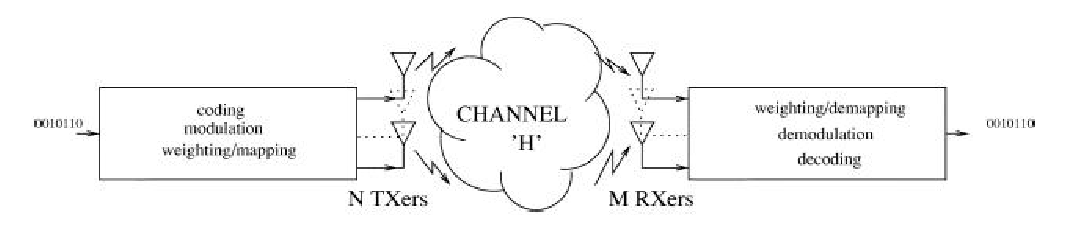
\includegraphics{Chapter1/Fig001.eps}
    \caption{Diagram of a wireless MIMO communication system}
    \label{fig:Fig1}
\end{figure}

\begin{figure}
    \centering
        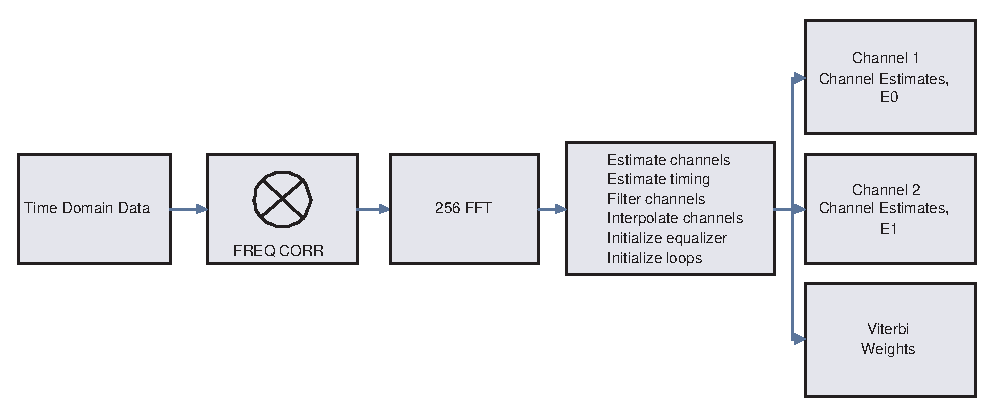
\includegraphics{Chapter1/Fig002.eps}
    \caption{Alamouti implementation in WiMAX}
    \label{fig:Fig2}
\end{figure}
